\chapter{Inverted pendulum analysis}


\section{Inverted pendulum description}
For this project an inverted pendulum set up is given. It consists of:
\begin{itemize}
	\item a DC motor
	\item a system of four gears linked by belt strap
	\item an arm
	\item a stick connected to the end of the arm with a liberty of movement of one degree
\end{itemize}

\begin{figure} [htbp]
	\centering
	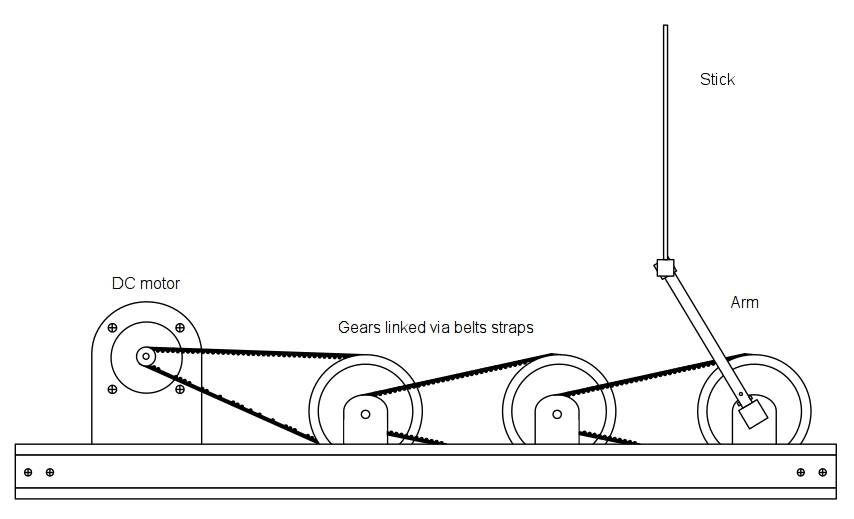
\includegraphics[width=0.8\linewidth]{figures/"Preanalysis&Requirement"/invertedPendulumDiagram}
	\caption{Diagram of the set up fully assembled} \label{fig:InvertedPendulumSetUp}
\end{figure}

\autoref{fig:InvertedPendulumSetUp} is a diagram of the set up when fully assembled. The DC motor moves the arm via the gears, a noteworthy fact is that out the four gears three are of the same size. This means that two gears do not have any influence on the torque and the angular velocity of the arm.

\section{Modelling of the Arm and Stick}
put the modelling section there

%%%%%%%%%%%%% Equation template %%%%%%%%%%%%%%%
%\begin{flalign}
%\hspace{30pt} & EQUATION1 &&& \text{[UNIT]} \notag \\
%& EQUATION2 &&& \text{[UNIT]} \label{eq:LABEL} 
%\end{flalign}
%\begin{description}
%  \item[\hspace{30pt}\textnormal{where:}]\hfill \\
%  \begin{tabular}{p{30pt}lp{250pt}l}
%& $x$ & TEXT & [UNIT]  \\
%& $y$ & VERY LONG TEXT THAT IS VERY LONG AND HAS A LOT OF WORDS IN IT YET THE FORMATTING STILL LOOKS NICE AND CLEAN AND EVERYTHING IS AWESOME & [UNIT]  \\
%& $z$ & TEXT & [UNIT]
%\end{tabular}
%\end{description}
%%%%%%%%%%%%%%%%%%%%%%%%%%%%%%%%%%%%%%%%%%%%%%%

\begin{flalign}
\hspace{30pt} & F_x=\ddot{x}_sM_s &&& \text{[N]} \notag \\
& F_y=\ddot{y}_sM_s &&& \text{[N]} \label{eq:FxFy} 
\end{flalign}
\begin{description}
  \item[\hspace{30pt}\textnormal{where:}]\hfill \\
  \begin{tabular}{p{30pt}lp{250pt}l}
& $F_x$ & is the force in the x direction. & [N]  \\
& $F_y$ & is the force in the y direction. & [N]  \\
& $x_s$ & is the position of the center of mass of the stick in the x direction. & [m] \\
& $y_s$ & is the position of the center of mass of the stick in the y direction. & [m]
\end{tabular}
\end{description}
text
\begin{flalign}
\hspace{30pt} & x_s=-l_a\sin (\theta_a)-\frac{l_s}{2} \sin (\theta_s) &&& \text{[m]} \notag \\
& y_s = l_a\cos (\theta_a)+\frac{l_s}{2} \cos(\theta_s) &&& \text{[m]} \label{eq:xsys} 
\end{flalign}
\begin{description}
  \item[\hspace{30pt}\textnormal{where:}]\hfill \\
  \begin{tabular}{p{30pt}lp{250pt}l}
& $l_a$ & is the length of the arm. & [m]  \\
& $l_s$ & is the length of the stick. & [m]  \\
& $\theta_a$ & is the angle between the arm and the y-axis. & [$^\circ$]  \\
& $\theta_s$ & is the angle between the stick and the y-axis. & [$^\circ$]
\end{tabular}
\end{description}
The derivative of $x_s$ and $y_s$ is found in equation \eqref{eq:diffxy}.
\begin{flalign}
\hspace{30pt} & \dot{x}_s=-l_a\dot{\theta}_a\cos(\theta_a)-\frac{l_s}{2}\dot{\theta}_s\cos(\theta_s) &&& \text{[m/s]} \notag \\
& \ddot{x}_s=-l_a\ddot{\theta}_a\cos(\theta_a)+l_a\dot{\theta}_a^2\sin(\theta_a)-\frac{l_s}{2}\ddot{\theta}_s\cos(\theta_s)+\frac{l_s}{2}\dot{\theta}_s^2\sin(\theta_s) &&& \text{[m/s$^2$]} \notag \\
& \dot{y}_s=-l_a \dot{\theta}_a\sin(\theta_a)-\frac{l_s}{2}\dot{\theta}_s\sin(\theta_s) &&& \text{[m/s]} \notag \\
& \ddot{y}_s=-l_a\ddot{\theta}_a\sin(\theta_a)-l_a\dot{\theta}_a^2\cos(\theta_a)-\frac{l_s}{2}\ddot{\theta}_s\sin(\theta_s)-\frac{l_s}{2}\dot{\theta}_s^2\cos(\theta_s) &&& \text{[m/s$^2$]} \label{eq:diffxy} 
\end{flalign}

The forces perpendicular to the stick at the center of mass is found by equation \eqref{eq:perpFxFy}.
\begin{flalign}
\hspace{30pt} & F_{px}=F_x\cos(\theta_s) &&& \text{[N]} \notag \\
& F_{py}=F_y\sin(\theta_s) &&& \text{[N]} \notag \\
& F_p = F_{px}+F_{py} &&& \text{[N]} \label{eq:perpFxFy}
\end{flalign}

Something about D'Alembert's law in equation \eqref{eq:Jsthetas}.
\begin{flalign}
\hspace{30pt} & J_s\ddot{\theta}_s=F_p\frac{l_s}{2}-\tau_f &&& \text{[N$\cdot$m]} \notag \\
& \tau_f =b_{as}\dot{\theta}_{as} &&& \text{[N$\cdot$m]} \label{eq:Jsthetas}
\end{flalign}
\begin{description}
  \item[\hspace{30pt}\textnormal{where:}]\hfill \\
  \begin{tabular}{p{30pt}lp{250pt}l}
& $J_s$ & is the moment of inertia for the stick & [kg$\cdot$m$^2$]  \\
& $\tau_f$ & is the torque of the friction acting on the stick & [N$\cdot$m] \\
& $b_{as}$ & is the viscous friction coefficient between the arm and the stick & [N$\cdot$m$\cdot$s] \\
& $\dot{\theta}_{as}$ & is the difference in velocity between the arm and the stick & [m/s]
\end{tabular}
\end{description}
\todo[author=Jacob, inline]{The units doesn't seem to match up.}

Inserting $F_p$ into equation \eqref{eq:Jsthetas} gives equation \eqref{eq:JsLong}
\begin{flalign}
\hspace{30pt} & J_s\ddot{\theta}_s=\frac{l_s}{2}\left(F_x\cos(\theta_s)+F_y\sin(\theta_s)\right)-b_{as}\dot{\theta}_{as} &&& \text{[N$\cdot$m]} \notag \\
& J_s\ddot{\theta}_s = \frac{l_s}{2}M_s \Big( -l_a\ddot{\theta}_a\left(\cos(\theta_a)\cos(\theta_s)+\sin(\theta_a)\sin(\theta_s)\right) && \notag \\
& \phantom{========} +l_a\dot{\theta}_a^2\left(\sin(\theta_a)\cos(\theta_s)-\cos(\theta_a)\sin(\theta_s)\right)  &&& \notag \\
& \phantom{========} -\frac{l_s}{2}\ddot{\theta}_s\left(\cos(\theta_s)\cos(\theta_s)+\sin(\theta_s)\sin(\theta_s)\right) &&& \notag \\
& \phantom{========} +\frac{l_s}{2}\dot{\theta}_s^2\left(\sin(\theta_s)\cos(\theta_s)-\cos(\theta_s)\sin(\theta_s)\right) &&& \notag \\
& \phantom{========}  +g\sin(\theta_s) \Big)-b_{as}\dot{\theta}_{as} &&& \text{[N$\cdot$m]} \label{eq:JsLong}
\end{flalign}

Using the trigonometric properties in equation \eqref{eq:trigprop}, equation \eqref{eq:JsLong} is shortened to equation \eqref{eq:JsShort}.
\begin{flalign}
\hspace{30pt} & \cos(\theta_a)\cos(\theta_s)\pm \sin(\theta_a)\sin(\theta_s)=\cos(\theta_a \mp \theta_s) &&& \notag \\
& \sin(\theta_a)\cos(\theta_s)\pm \cos(\theta_a)\sin(\theta_s) = \sin(\theta_a \pm \theta_s) &&& \notag \\ 
& \cos(\theta_s)^2+\sin(\theta_s)^2=1 &&& \label{eq:trigprop}
\end{flalign}

\begin{flalign}
\hspace{30pt} & J_s\ddot{\theta}_s = \frac{l_s}{2}M_s \Big( -l_a\ddot{\theta}_a \cos(\theta_a-\theta_s)+l_a\dot{\theta}_a^2 \sin(\theta_a-\theta_s)  &&& \notag \\
& \phantom{========} -\frac{l_s}{2}\ddot{\theta}_s +g\sin(\theta_s) \Big)-b_{as}\dot{\theta}_{as} &&& \text{[N$\cdot$m]} \label{eq:JsShort}
\end{flalign}

Linearization using first order taylor approximation [insert ref to note in google drive]. Something about multiple variables.
\begin{flalign}
\hspace{30pt} & f\left(\theta_a, \dot{\theta}_a, \ddot{\theta}_a, \theta_s, \ddot{\theta}_s\right) \approx f\left(\bar{\theta}_a, 0, 0, \bar{\theta}_s, 0\right) + \left. \frac{\partial f}{\partial \theta_a}\right|_{(\bar{\theta}_a, \bar{\theta}_s)} \hat{\theta}_a &&& \notag \\
& \phantom{===========.} + \left. \frac{\partial f}{\partial \dot{\theta}_a}\right|_{(\bar{\theta}_a, \bar{\theta}_s)} \hat{\dot{\theta}}_a + \left. \frac{\partial f}{\partial \ddot{\theta}_a}\right|_{(\bar{\theta}_a, \bar{\theta}_s)} \hat{\ddot{\theta}}_a &&& \notag \\
& \phantom{===========.} + \left. \frac{\partial f}{\partial \theta_s}\right|_{(\bar{\theta}_a, \bar{\theta}_s)} \hat{\theta}_s + \left. \frac{\partial f}{\partial \ddot{\theta}_s}\right|_{(\bar{\theta}_a, \bar{\theta}_s)} \hat{\ddot{\theta}}_s &&& \text{[$\cdot$]}\label{eq:1stTaylor}
\end{flalign}

The 3 terms with sin or cos in equation \eqref{eq:JsShort} will be approximated individually using equation \eqref{eq:1stTaylor} remembering that $\bar{\theta}=\bar{\dot{\theta}}=\bar{\ddot{\theta}}=0$.
\begin{flalign}
\hspace{30pt} & -l_a\ddot{\theta}_a\cos\left(\theta_a-\theta_s\right) \approx 0 + l_a\bar{\ddot{\theta}}_a\sin\left(\bar{\theta}_a-\bar{\theta}_s\right)\hat{\theta}_a &&& \notag \\ 
& \phantom{============} -l_a\cos\left(\bar{\theta}_a-\bar{\theta}_s\right)\hat{\ddot{\theta}}_a - l_a\bar{\ddot{\theta}}_a\sin\left(\bar{\theta}_a-\bar{\theta}_s\right)\hat{\theta}_s &&& \notag \\
& -l_a\ddot{\theta}_a\cos\left(\theta_a-\theta_s\right) \approx -l_a\hat{\ddot{\theta}}_a &&&
\end{flalign} %\bar{\ddot{\theta}}_s
\begin{flalign}
\hspace{30pt} & l_a\dot{\theta}_a^2\sin\left(\theta_a-\theta_s\right) \approx 0 + l_a\bar{\dot{\theta}}_a^2\cos\left(\bar{\theta}_a-\bar{\theta}_s\right)\hat{\theta}_a &&& \notag \\
& \phantom{==========.} + 2l_a\bar{\dot{\theta}}_a\sin\left(\bar{\theta}_a-\bar{\theta}_s\right)\hat{\dot{\theta}}_a-l_a\bar{\dot{\theta}}_a^2\cos\left(\bar{\theta}_a-\bar{\theta}_s\right)\hat{\theta}_s &&& \notag \\
& l_a\dot{\theta}_a^2\sin\left(\bar{\theta}_a-\bar{\theta}_s\right) \approx 0 &&&
\end{flalign}
\begin{flalign}
\hspace{30pt} & g\sin\left(\theta_s\right) \approx g\sin\left(\bar{\theta}_s\right) +g\cos\left(\bar{\theta}_s\right)\hat{\theta}_s &&& \notag \\
& g\sin\left(\theta_s\right) \approx g\hat{\theta}_s &&& 
\end{flalign}

Inserting the linearized terms in equation \eqref{eq:JsShort} and using the moment of inertia for a rotating stick, $J_s=\frac{1}{12}M_sl_s^2$, the linearized model becomes \eqref{eq:JsFinal}.
\begin{flalign}
\hspace{30pt} & \frac{1}{12}M_sl_s^2\ddot{\theta}_s=\frac{l_s}{2}M_s\left(-l_a\ddot{\theta}_a-\frac{l_s}{2}\ddot{\theta}_s+g\theta_s\right)-b_{as}\dot{\theta}_{as} &&& \notag \\
& \frac{1}{12}M_sl_s^2\ddot{\theta}_s+\frac{1}{4}M_sl_s^2\ddot{\theta}_s=\frac{l_s}{2}M_s\left(-l_a\ddot{\theta}_a+g\theta_s\right)-b_{as}\dot{\theta}_{as} &&& \notag \\
& \frac{1}{3}M_sl_s^2\ddot{\theta}_s=\frac{l_s}{2}M_s\left(-l_a\ddot{\theta}_a+g\theta_s\right)-b_{as}\dot{\theta}_{as} &&& \notag \\
& \ddot{\theta}_s=\frac{3}{2l_s}\left(-l_a\ddot{\theta}_a-\frac{l_s}{2}\ddot{\theta}_s+g\theta_s\right)-\frac{3b_{as}\left(\dot{\theta}_s-\dot{\theta}_a\right)}{M_sl_s^2} &&& \text{[N$\cdot$m]} \label{eq:JsFinal}
\end{flalign}

Laplace transform
\begin{flalign}
\hspace{30pt} & s^2\Theta_s=\frac{3}{2l_s}\left(-s^2l_a\Theta_a+g\Theta_s\right)-s\frac{3b_{as}}{M_sl_s^2}\Theta_s+s\frac{3b_{as}}{M_sl_s^2}\Theta_a &&& \notag \\
& \Theta_s\left(s^2+\frac{3b_{as}}{M_sl_s^2}s-\frac{3g}{2l_s}\right)=\Theta_a\left(-\frac{3l_a}{2l_s}s^2+\frac{3b_{as}}{M_sl_s^2}s\right) &&& \notag \\
& \frac{\Theta_s}{\Theta_a}=-\frac{\frac{3l_a}{2l_s}s^2-\frac{3b_{as}}{M_sl_s^2}s}{s^2+\frac{3b_{as}}{M_sl_s^2}s-\frac{3g}{2l_s}}
\end{flalign}
